\chapter{Optical modeling}
\label{chapter:optical_modeling}

The main components of the measurement cell are phototransistor (PT), source of light (emitter) and photobarrier (PB). 
The purpose of the chapter is to find the function $F = f(I_{pt})$, which describes the relation between current on the phototransistor $I_{pt}$ and force $F$, applied to the barrier.

The current on PT depends on the Illuminance at the phototransistor area. 
For the project I use a PT module (EE-SX1321, OMRON), it consists of a set of receiver' and emitter' cells \cite[Fig. 4]{my_love_pressure_photosensor}.
Therefore, I will calculate the radiant flux for each cell separately.

Optical model of my measurement cell wil be based on the one described in \cite{my_love_pressure_photosensor}.

In the chapter, PB will be simplified to the spring element with aperture. When a force is applied to the PB, the aperture will be shifted relative to the main optical axis of the light source.


Limitations of the mathematical model:
\begin{itemize}
    \item LED is Lambert's source of light.
    \item PT acceptable wavelength is the same as of emitted light.
    \item Light is a stream of particles.
    \item PB will be simplified to the spring element with aperture. When a force is applied to the PB, the aperture will be shifted relative to the main optical axis of the light source.
\end{itemize}


Lets start with emitter - in the project the emitter device is light-emitting diode (LED). The device is a semiconductor which transforms electrical power into light \cite{LED_flux_estimation}.

\section{Simplified model}

The force measurement cell can be simplified to model of an spring with barrier and optocoupler.

% ------------------------------------------
% Illuminance
Radiant intensity on a unit area of the phototransistor:

\[R^2 = (s_1- x)^2 + (s_2 - y)^2 + l_0 ^2\\

h = |y - s_2|\\

\beta = \arcsin(\frac{h}{\sqrt{R}})\\

I = I_0 * \frac{l_0 \cos{\beta}}{2 \pi R}\]

$R$ - radius vector from $i$-th light source to the $j$-th receiver cell,

$\beta$ - angle between norm vector of emitter area and the vector R,

$s_1, s_2$ - coordinates of the LED,

$x, y$ - coordinates of the PT,


\begin{figure}[H]
    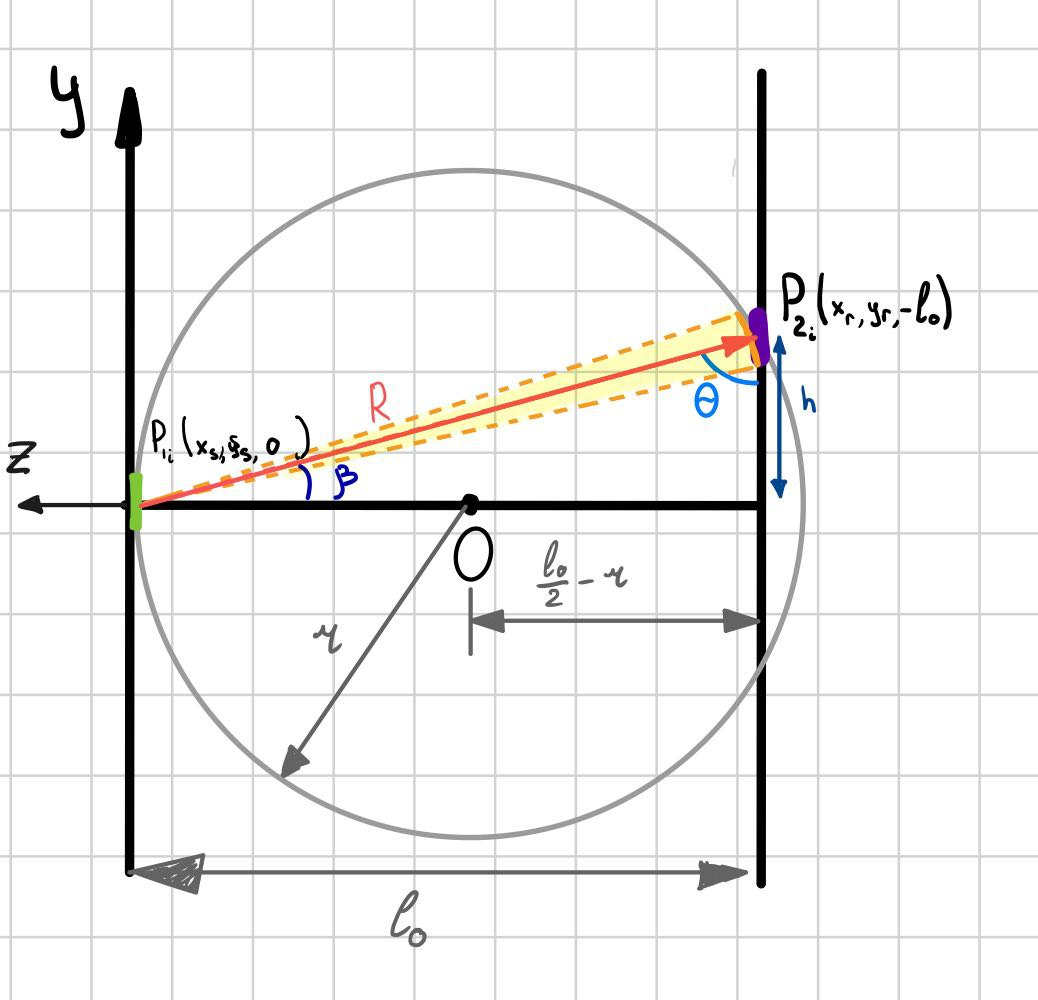
\includegraphics[width=0.5\textwidth]{figs/simplified_model_notebook.jpg}
      \centering
      \caption{The geometrical relationships between LED (green) and PT(purple)}
      \label{fig:simplified_model_notebook}
    \end{figure}
    
\begin{figure}[H]
    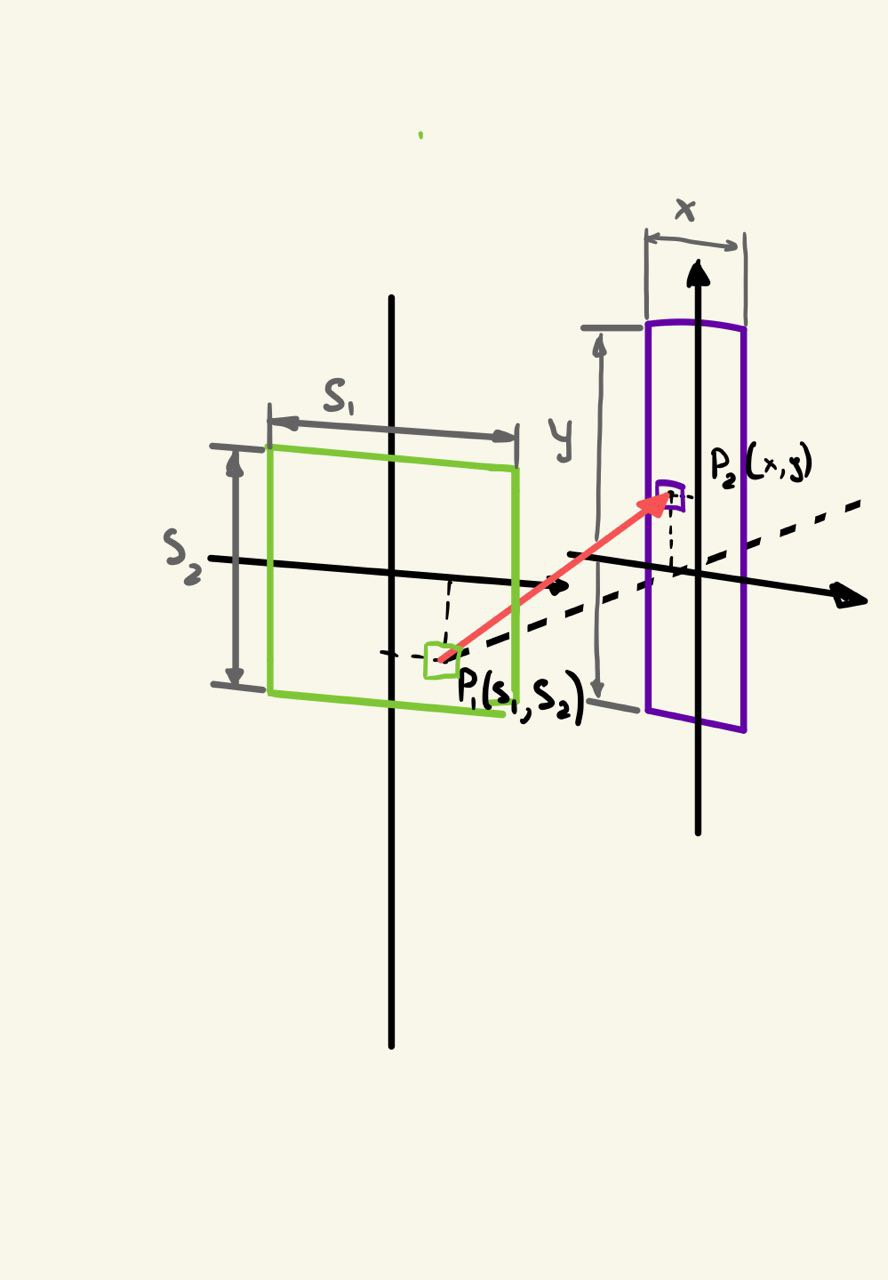
\includegraphics[width=0.5\textwidth]{figs/arrangement_of_LED_PT.jpg}
        \centering
        \caption{LED (green) and photoreceiver (purple) arrangement} 
        \label{fig:arrangement_of_LED_PT}
    \end{figure}
    
\begin{figure}[H]
    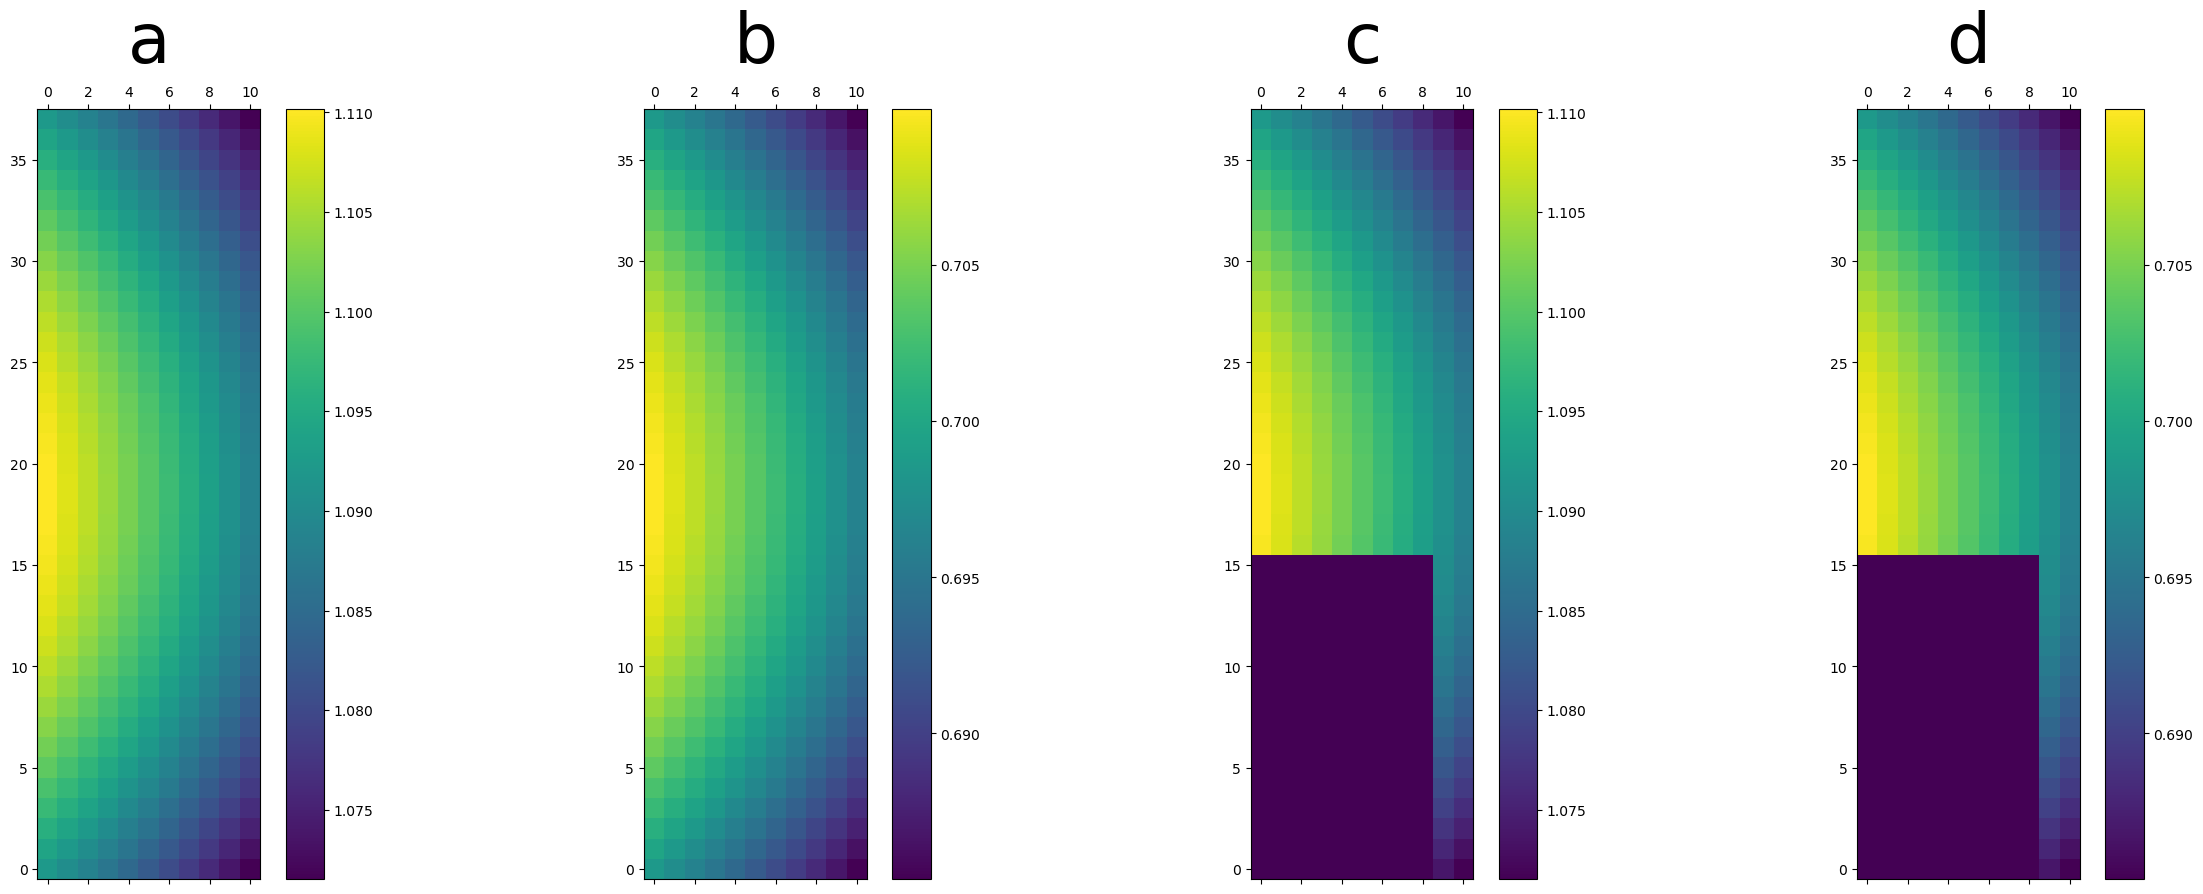
\includegraphics[width=1\textwidth]{figs/intensity_output.png}
      \centering
      \caption{Photoreceiver intensity from the formulas: a. The intensity of the }
      \label{fig:intensity_output}
    \end{figure}
    
% -------------------------------------------

How to calculate the light intensity on the receiver area (flux)?

The model should include area of the emitter and receiver since we measure the current change on the PT

Illuminance estimates the flux received by some area. 




% \section{Source code file structure}

% % Every EO file starts with meta-information, which includes:
% \begin{itemize}
%     \item package — the namespace where all declared objects are located. Other files use the package to refer to objects located in the file. This construct has a form of \ff{+package <package name>}.
%     \item aliases — fully-qualified names (FQN for short) (package plus object name) used to import other definitions to the current file. This construct has a form of \ff{+alias <FQN of object>}.
% \end{itemize}

% Example of meta-information block:

% \begin{ffcode}
% +package main
% +alias org.eolang.txt.sprintf
% \end{ffcode}

% Then declarations follow, which are the main construction blocks of EO programs.

% Literal values syntax is built into EO, and contains:
% \begin{itemize}
%     \item \ff{"str"} for strings
%     \item \ff{42} for integers
%     \item \ff{4.2} for floating-point numbers
%     \item \ff{'c'} for single characters
%     \item \ff{AB-42} for bytes sequences (hexadecimal representation of bytes delimited by dashes).
% \end{itemize}

% Booleans are implemented in the standard library, they are objects.

% Objects have the following syntax:

% \begin{ffcode}
% [free_attr_1 free_attr_2, optional_var_attr...] > object_name
%     <expr> > bound_attr_1
%     <expr> > bound_attr_2
%     seq > @
%         <imperative operation 1>
%         <imperative operation 2>
%         <result expr>
% \end{ffcode}

% where:
% \begin{itemize}
%     \item free attributes, marked as \ff{<free\_attr>}, are similar to arguments in traditional languages.
%     \item bound attributes, marked as \ff{<bound\_attr>}, are entries holding an expression \ref{section:immutability_of_data_in_eo}. They are logically similar to the assignment in conventional OOP languages. Though, they can not be reassigned and do not evaluate until their result is \textit{dataized}, e.g., computed, transformed from a declaration to a particular value by one of the imperative operations, such as print.
%     \item expressions, marked as \ff{<expr>}, take a form of:
% \begin{ffcode}
% number1.add
%     number2
% \end{ffcode}
%           or 
% \begin{ffcode}
% add.
%     number1
%     number2
% \end{ffcode}
%     both of which are semantically equivalent.

%     Like with attributes, to which they can be bound, expressions are not evaluated until the result is dataized.

%     Object declaration is an object as well, which means such constructions can be nested.
%     \item \ff{... > @} marks the \textit{decoration} operation: in a nutshell, it takes the referenced object (marked as \ff{...}) and wraps it with additional attributes specified in the object. This provides an approach to implementing the singular inheritance of objects.
    
%     For example, in the following snippet, object \ff{B}, which decorates \ff{A}, will contain both \ff{first} and \ff{second} as its bound attributes:

%     \begin{ffcode}
% [] > A
%   1 > first

% [] > B
%   A > @
%   2 > second
%     \end{ffcode}

%     The meaning of \ff{seq} will be discussed later.
% \end{itemize}

% These are all EO built-in mechanisms. It can be seen that EO does not have built-in classes. The implementation of the class framework will be described later in the text.

% The powerful part of EO lies in its atoms. It is not possible to write a program in EO without atoms because dataization can only happen there. And without dataization, the program is a bare declaration, not differing semantically from YAML or JSON.

% Atoms include both functions (i.e., print) and data objects, most notable of them are:
% \begin{itemize}
%   \item booleans,
%   \item \ff{memory} object that allows to store mutable primitive values, including strings, numbers, characters and bytes,
%   \item \ff{cage} object that allows to store objects,
%   \item \ff{seq} function that allows sequential computation.
% \end{itemize}

% One particular atom that is very important to this project is \ff{seq}: it provides a way to express imperative computation in EO. It works by accepting an arbitrary number of expressions as arguments. All except the last one are dataized to actually perform the computation. The last expression is returned as-is because dataized expressions yield a primitive value, which does not have the original structure, original nested attributes and are practically useless for further operations. The final dataization usually happens in \ff{print} operation or other atoms performing side effects.

% \ff{seq} allows objects to simulate function behavior from traditional languages. In this text, I will refer to objects with \ff{seq} block as \textbf{functions}. While this is not entirely correct syntactically, this will ease the reading of the text, as \textbf{function} is a widely-used term for such construction.


% \section{Internal representation of compiled EOLANG programs}

% EOLANG is essentially a $\varphi$-calculus wrapped into a programming language, with a convenient syntax for writing programs on a standard computer keyboard. It also includes features that make it useful for general-purpose tasks, such as the I/O library, math library, built-in data structures, etc.

% EO compiler outputs Java source code which creates a phi-calculus graph that describes the program. This fact affects the boundaries of allowed modifications to EOLANG, as we can't implement features that do not correspond to phi-calculus.


% \section{Analysis of EO suitability for the goal of this project}

% EO focuses on pure objects, but the term "pure" may be extended to OOP languages as well. With respect to object-oriented languages, this term means that the following conditions hold \cite{making_pure_oop_languages_practical,why_java_is_not_pure}:

% % TODO: reformat this
% % TODO: move this to EO analysis section
% \begin{itemize}
%     \item (1) Language provides Encapsulation/Data Hiding;
%     \item (2) Language provides Inheritance;
%     \item (3) Language provides Polymorphism;
%     \item (4) Language provides Abstraction;
%     \item (5) All predefined types in the language are objects;
%     \item (6) All user-defined types in the language are objects;
%     \item (7) All operations performed on objects must be only through methods exposed at the objects.
% \end{itemize}

% Having a pure language facilitates richer static analysis, as the amount of uncontrolled side effects \cite{gifford1986integrating} is minimized, and they can be analyzed. The main goal of the project is to provide the most suitable representation for further static analysis, thus, checking these properties is essential.

% \subsection{How do these seven properties ease static analysis?}

% First, it is important to check how these properties help to improve the quality of static analysis and is it worth to fulfill them.

% \begin{itemize}
%   \item Encapsulation allows skipping the check of external direct data access, as it hides the data behind functions. As such, data access should only be checked inside the class declaration.
%   \item Inheritance, polymorphism, and abstraction do not help with analysis, they are designed to help developers.
%   \item Defining built-in types as language objects helps by minimizing the analyzer's built-in logic, as this logic may be deduced from the source code of the standard library.
%   \item Defining all user types as objects helps by removing handling of custom type logic; all analysis focuses on objects solely.
%   \item Shrinking range of object manipulation to only methods exposed by the object itself plays the same role as encapsulation: analyzer does not have to consider external object manipulation other than the logic defined in the class itself.
% \end{itemize}

% Four of seven properties make sense to fulfill to reach the goal of the project, so I will focus on them.


% \subsection{Checking EO against pure OOP language properties}

% \subsubsection{Encapsulation/Data Hiding}

% EOLANG paper \cite{eolang_phi_calculus} states that the language does not support encapsulation/data hiding, this property is missing.

% \subsubsection{Predefined types are objects}
% Objects are the main focus of the EO language, there are only objects. Literals are represented as objects as well. This property is fulfilled.

% \subsubsection{User-defined types are objects}
% Same as with predefined types, there is no way to define non-object types.

% \subsubsection{Methods defined on the object are the only ways of object manipulation}
% Since there is no assignment in EO and the only type is the object, the only way to interact with objects is to call its methods.

% \subsubsection{Conclusion}
% Three of the defined properties hold for EO. Thus, it makes sense to fulfill them in the project.


% \section{Phi-calculus overview}
% \label{section:phi_calculus}

% $\varphi$-calculus \cite{eolang_phi_calculus} is based on lambda-calculus, formulated by A. Church \cite{church2001logic} and set theory. The simplified description of underlying calculus is given to facilitate a better understanding of EOLANG hard boundaries.

% \subsection{Objects}
% The core entity of $\varphi$-calculus is an object. Object $o$ is a set of ordered pairs named \emph{attributes} such that keys $a$ are identifiers and values $v$ are objects. An identifier may be one of the reserved meaningful values: $\varphi$, $\rho$, $\sigma$, $v$, or any text without spaces starting with a lower-case English letter:

% \[
%     o = \{(a_1, v_1), (a_2, v_2), ..., (a_i, v_i)\}, \textnormal{ where } i \in [0, \infty)
% \]

% Empty objects are allowed. An empty object is denoted by $\varnothing$, as in classic set theory.

% The \emph{scope} of an object $o = \{(a_1, v_1), ..., (a_i, v_i)\}$ is denoted with $\hat{o}$ and is a set of $a_1, ..., a_i$.

% The \emph{arity} of an object $o$ is the cardinality of its scope and is represented as $|\hat{o}|$.

% From the description of the object, it is clear that $\varphi$-calculus was designed by a developer for developers --- multi-character identifiers are first-class units, unlike in mathematics. Thus, treating it as a programming language notation instead of a mathematical notation may help to understand this calculus better.

% \subsection{Data}
% The indivisible unit of $\varphi$-calculus is \emph{data} --- the possible values of data depend on the implementation platform, but generally-available types include integer numbers, floating-point numbers, strings, bytes, byte sequences and booleans. Data is an object as well. For the purposes of this project, available data types are the ones available in the EOLANG compiler. For the list, refer to chapter \ref{chapter:eo_overview}.

% \subsection{Attributes}
% Attributes are divided into two types:

% \begin{itemize}
%     \item \emph{free attributes} --- attributes which have $\varnothing$ as a value. Formally, attribute $a$ of object $o$ is free iff $(a, \varnothing) \in o$.

%     \item \emph{bound attributes} --- attributes which have non-empty set as a value. Formally, attribute $a$ of object $o$ is bound iff $\exists (a, v) \in o$ where $v \notin o$.
% \end{itemize}

% \subsubsection{Accessing attributes}
% If object $o$ has an attribute named $a$ that contains value $v$ (formally --- $\exists (a, v) \in o$, for example, $o = \{ (a, v) \}$), then $v$ may be accessed using dot notation: $o.a$.

% Dot notation may be chained if $v$ is an object as well. $v$ in the following example may be accessed with $o.a.b$:

% \[ o = \{ (a, \{(b, v)\}) \} \]

% Both bound and free attributes may be accessed this way.

% \subsection{Abstraction}
% If an object contains at least one free attribute, it is named \emph{abstract object}. The process of creation of an abstract object is called \emph{abstraction}.

% If an object contains no free attributes, it is named \emph{closed object}.

% \subsection{Application}
% Application is an operation defined on abstract objects that creates a new object with one or more free attributes becoming bound. Formally, if $x$ is an abstract object and $y$ is object with $\hat{y} \subseteq \hat{x}$, then the resulting object $o$ will contain pairs with values as follows:

% \[
%     \left(
%         a \in \hat{x}, v =
%         \begin{cases}
%             x.a \textnormal{ if } x.a \neq \varnothing \\
%             y.a \textnormal{ if } x.a = \varnothing
%         \end{cases}
%     \right)
% \]

% If not all attributes become bound after application, the newly created object is abstract, otherwise --- the newly created object is closed.

% \subsection{Parent and home objects}
% J2EO does not use parent and home objects, but they are still present in this description since they may facilitate new feature implementation in the future.

% For object $o$, $o.\rho$ represents its \emph{parent} object, i.e., the object that created $o$.

% For object $o$, $o.\sigma$ represents its \emph{home} object, i.e., the parent object of abstract object from which $o$ was created.

% % TODO: maybe add examples of arrow-notation here like in Yegor's paper?

% \subsection{Decoration}
% The decoration is the core operation of $\varphi$-calculus. \emph{Decoratee} is denoted with $\varphi$; this symbol gives the name to $\varphi$-calculus. \emph{Decoration} is the operation which extends object $o$ with additional attributes to produce new object $x$. This operation is similar to inheritance in object-oriented programming languages.

% An example of using decoration where B decorates A:

% \[
%     A = \{ (\texttt{a}, 42) \} \\
%     B = \{ (\varphi, A) \}  \quad\equiv\quad  B = \{ (\varphi, \{ (\texttt{a}, 42) \}) \} \\
% \]

% % TODO: Add an example?

% \subsection{Atoms}
% Atoms are defined by the runtime, and thus, described in the EOLANG description --- the runtime used by J2EO.

% \subsection{Locators}
% $\varphi$-calculus is used to represent source code, which often spans across several files and may contain thousands of object declarations, some of which are named with the same identifier. To deterministically resolve such conflicts, $\varphi$-calculus contains \emph{locators} --- sequence of identifiers separated with a dot. $\Phi$ denotes a root object --- all top-level object declarations are bound to it.

% \subsection{Identity}
% $\varphi$-calculus is used to represent abstract entities, and as such, objects should contain a built-in identity. For object $o$, $o.v$ is a positive integer data object that is unique to $o$ in the entire runtime scope. There's no guarantee that this number is always the same across different environments and executions, but it strictly stays the same after the object is created.

% \subsection{Summary}

% To sum up, $\varphi$-calculus covers types, objects, and operations on them, providing all facilities to implement the general semantics of Java programs.
